% Options for packages loaded elsewhere
\PassOptionsToPackage{unicode}{hyperref}
\PassOptionsToPackage{hyphens}{url}
%
\documentclass[
]{article}
\usepackage{amsmath,amssymb}
\usepackage{iftex}
\ifPDFTeX
  \usepackage[T1]{fontenc}
  \usepackage[utf8]{inputenc}
  \usepackage{textcomp} % provide euro and other symbols
\else % if luatex or xetex
  \usepackage{unicode-math} % this also loads fontspec
  \defaultfontfeatures{Scale=MatchLowercase}
  \defaultfontfeatures[\rmfamily]{Ligatures=TeX,Scale=1}
\fi
\usepackage{lmodern}
\ifPDFTeX\else
  % xetex/luatex font selection
\fi
% Use upquote if available, for straight quotes in verbatim environments
\IfFileExists{upquote.sty}{\usepackage{upquote}}{}
\IfFileExists{microtype.sty}{% use microtype if available
  \usepackage[]{microtype}
  \UseMicrotypeSet[protrusion]{basicmath} % disable protrusion for tt fonts
}{}
\makeatletter
\@ifundefined{KOMAClassName}{% if non-KOMA class
  \IfFileExists{parskip.sty}{%
    \usepackage{parskip}
  }{% else
    \setlength{\parindent}{0pt}
    \setlength{\parskip}{6pt plus 2pt minus 1pt}}
}{% if KOMA class
  \KOMAoptions{parskip=half}}
\makeatother
\usepackage{xcolor}
\usepackage[margin=1in]{geometry}
\usepackage{color}
\usepackage{fancyvrb}
\newcommand{\VerbBar}{|}
\newcommand{\VERB}{\Verb[commandchars=\\\{\}]}
\DefineVerbatimEnvironment{Highlighting}{Verbatim}{commandchars=\\\{\}}
% Add ',fontsize=\small' for more characters per line
\newenvironment{Shaded}{}{}
\newcommand{\AlertTok}[1]{\textcolor[rgb]{1.00,0.00,0.00}{\textbf{#1}}}
\newcommand{\AnnotationTok}[1]{\textcolor[rgb]{0.38,0.63,0.69}{\textbf{\textit{#1}}}}
\newcommand{\AttributeTok}[1]{\textcolor[rgb]{0.49,0.56,0.16}{#1}}
\newcommand{\BaseNTok}[1]{\textcolor[rgb]{0.25,0.63,0.44}{#1}}
\newcommand{\BuiltInTok}[1]{\textcolor[rgb]{0.00,0.50,0.00}{#1}}
\newcommand{\CharTok}[1]{\textcolor[rgb]{0.25,0.44,0.63}{#1}}
\newcommand{\CommentTok}[1]{\textcolor[rgb]{0.38,0.63,0.69}{\textit{#1}}}
\newcommand{\CommentVarTok}[1]{\textcolor[rgb]{0.38,0.63,0.69}{\textbf{\textit{#1}}}}
\newcommand{\ConstantTok}[1]{\textcolor[rgb]{0.53,0.00,0.00}{#1}}
\newcommand{\ControlFlowTok}[1]{\textcolor[rgb]{0.00,0.44,0.13}{\textbf{#1}}}
\newcommand{\DataTypeTok}[1]{\textcolor[rgb]{0.56,0.13,0.00}{#1}}
\newcommand{\DecValTok}[1]{\textcolor[rgb]{0.25,0.63,0.44}{#1}}
\newcommand{\DocumentationTok}[1]{\textcolor[rgb]{0.73,0.13,0.13}{\textit{#1}}}
\newcommand{\ErrorTok}[1]{\textcolor[rgb]{1.00,0.00,0.00}{\textbf{#1}}}
\newcommand{\ExtensionTok}[1]{#1}
\newcommand{\FloatTok}[1]{\textcolor[rgb]{0.25,0.63,0.44}{#1}}
\newcommand{\FunctionTok}[1]{\textcolor[rgb]{0.02,0.16,0.49}{#1}}
\newcommand{\ImportTok}[1]{\textcolor[rgb]{0.00,0.50,0.00}{\textbf{#1}}}
\newcommand{\InformationTok}[1]{\textcolor[rgb]{0.38,0.63,0.69}{\textbf{\textit{#1}}}}
\newcommand{\KeywordTok}[1]{\textcolor[rgb]{0.00,0.44,0.13}{\textbf{#1}}}
\newcommand{\NormalTok}[1]{#1}
\newcommand{\OperatorTok}[1]{\textcolor[rgb]{0.40,0.40,0.40}{#1}}
\newcommand{\OtherTok}[1]{\textcolor[rgb]{0.00,0.44,0.13}{#1}}
\newcommand{\PreprocessorTok}[1]{\textcolor[rgb]{0.74,0.48,0.00}{#1}}
\newcommand{\RegionMarkerTok}[1]{#1}
\newcommand{\SpecialCharTok}[1]{\textcolor[rgb]{0.25,0.44,0.63}{#1}}
\newcommand{\SpecialStringTok}[1]{\textcolor[rgb]{0.73,0.40,0.53}{#1}}
\newcommand{\StringTok}[1]{\textcolor[rgb]{0.25,0.44,0.63}{#1}}
\newcommand{\VariableTok}[1]{\textcolor[rgb]{0.10,0.09,0.49}{#1}}
\newcommand{\VerbatimStringTok}[1]{\textcolor[rgb]{0.25,0.44,0.63}{#1}}
\newcommand{\WarningTok}[1]{\textcolor[rgb]{0.38,0.63,0.69}{\textbf{\textit{#1}}}}
\usepackage{longtable,booktabs,array}
\usepackage{calc} % for calculating minipage widths
% Correct order of tables after \paragraph or \subparagraph
\usepackage{etoolbox}
\makeatletter
\patchcmd\longtable{\par}{\if@noskipsec\mbox{}\fi\par}{}{}
\makeatother
% Allow footnotes in longtable head/foot
\IfFileExists{footnotehyper.sty}{\usepackage{footnotehyper}}{\usepackage{footnote}}
\makesavenoteenv{longtable}
\usepackage{graphicx}
\makeatletter
\def\maxwidth{\ifdim\Gin@nat@width>\linewidth\linewidth\else\Gin@nat@width\fi}
\def\maxheight{\ifdim\Gin@nat@height>\textheight\textheight\else\Gin@nat@height\fi}
\makeatother
% Scale images if necessary, so that they will not overflow the page
% margins by default, and it is still possible to overwrite the defaults
% using explicit options in \includegraphics[width, height, ...]{}
\setkeys{Gin}{width=\maxwidth,height=\maxheight,keepaspectratio}
% Set default figure placement to htbp
\makeatletter
\def\fps@figure{htbp}
\makeatother
\setlength{\emergencystretch}{3em} % prevent overfull lines
\providecommand{\tightlist}{%
  \setlength{\itemsep}{0pt}\setlength{\parskip}{0pt}}
\setcounter{secnumdepth}{-\maxdimen} % remove section numbering
\ifLuaTeX
  \usepackage{selnolig}  % disable illegal ligatures
\fi
\usepackage{bookmark}
\IfFileExists{xurl.sty}{\usepackage{xurl}}{} % add URL line breaks if available
\urlstyle{same}
\hypersetup{
  hidelinks,
  pdfcreator={LaTeX via pandoc}}

\author{}
\date{}

\begin{document}

\section{SLR Project P4 --- Distributed MapReduce Final
Documentation}\label{slr-project-p4-distributed-mapreduce-final-documentation}

\textbf{Project:} Custom distributed MapReduce in Go over remote lab
machines (\texttt{*.enst.fr})\\
\textbf{Repository:} \texttt{slr\_map\_reduce}\\
\textbf{Last updated:} 2026-07-01

\begin{center}\rule{0.5\linewidth}{0.5pt}\end{center}

\subsection{1. Executive Summary}\label{executive-summary}

This project implements a fault-tolerant batch MapReduce framework with:

\begin{itemize}
\tightlist
\item
  A Go orchestrator (\texttt{scripts/mapreduce}) that deploys workers,
  drives phases, and merges outputs.
\item
  HTTP workers (\texttt{scripts/worker}) that execute map/reduce,
  partition intermediate data by hash, and exchange buckets.
\item
  Pluggable jobs implementing \texttt{mrjob.Mapper} /
  \texttt{mrjob.Reducer} (\texttt{scripts/jobs/*}).
\item
  A Kafka Streams baseline (\texttt{kafka/*}) to compare compute time
  and operational trade-offs.
\end{itemize}

Three additional use-case jobs were implemented and validated
end-to-end:

\begin{enumerate}
\def\labelenumi{\arabic{enumi}.}
\tightlist
\item
  \texttt{langdetect} --- language distribution via stop-word scoring.
\item
  \texttt{domainpop} --- domain popularity from \texttt{WARC-Target-URI}
  headers.
\item
  \texttt{docdensity} --- document size and character-density counters.
\end{enumerate}

All reducers emit integer strings to remain compatible with the
orchestrator's integer-sum merge.

\begin{center}\rule{0.5\linewidth}{0.5pt}\end{center}

\subsection{2. Architecture}\label{architecture}

\subsubsection{2.1 Components}\label{components}

\begin{longtable}[]{@{}
  >{\raggedright\arraybackslash}p{(\columnwidth - 4\tabcolsep) * \real{0.3333}}
  >{\raggedright\arraybackslash}p{(\columnwidth - 4\tabcolsep) * \real{0.3333}}
  >{\raggedright\arraybackslash}p{(\columnwidth - 4\tabcolsep) * \real{0.3333}}@{}}
\toprule\noalign{}
\begin{minipage}[b]{\linewidth}\raggedright
Component
\end{minipage} & \begin{minipage}[b]{\linewidth}\raggedright
Path
\end{minipage} & \begin{minipage}[b]{\linewidth}\raggedright
Responsibility
\end{minipage} \\
\midrule\noalign{}
\endhead
\bottomrule\noalign{}
\endlastfoot
Orchestrator & \texttt{scripts/mapreduce} & Build worker with selected
job, deploy to hosts, run load→map→reduce→collect, merge final output \\
Worker & \texttt{scripts/worker} & Expose HTTP API, map local
chunks/files, write hash-partitioned buckets, fetch peers, reduce,
return result \\
Job API & \texttt{scripts/mrjob/api.go} & Defines \texttt{KeyValue},
\texttt{Mapper}, \texttt{Reducer} interfaces \\
Jobs & \texttt{scripts/jobs/*} & Independent map/reduce logic selected
with \texttt{-job} \\
Host discovery & \texttt{scripts/make\_hosts} & Build runtime host lists
from lab availability \\
Kafka baseline & \texttt{kafka/*} & Rootless KRaft deploy + cleanup +
Streams wordcount driver \\
\end{longtable}

\subsubsection{2.2 End-to-end lifecycle}\label{end-to-end-lifecycle}

\begin{enumerate}
\def\labelenumi{\arabic{enumi}.}
\tightlist
\item
  Parse flags (\texttt{-hosts}, \texttt{-job}, \texttt{-input} or
  \texttt{-commoncrawl}, \texttt{-n}, etc.).
\item
  Build worker binary with generated job binding
  (\texttt{job\_binding\_generated.go}).
\item
  Deploy the worker binary only to the initial active hosts and start
  remote \texttt{mr\_worker} with PID tracking.
\item
  Health-check those active workers (\texttt{/health}) until \texttt{N}
  slots are filled; keep the remaining discovered hosts as cold spares.
\item
  Load inputs (\texttt{POST\ /data} for local chunks,
  \texttt{POST\ /load} for WET URLs).
\item
  Run map (\texttt{POST\ /map}) where each worker writes bucket files
  partitioned by reducer.
\item
  Run reduce (\texttt{POST\ /reduce}) where each reducer pulls exactly
  one bucket from each peer.
\item
  Collect (\texttt{GET\ /result}) and merge counts in orchestrator.
\item
  If a slot host fails, deploy and health-check a cold spare on demand
  before replaying the needed phases for that slot.
\item
  Cleanup remote workers on every host that was actually started.
\end{enumerate}

\subsubsection{2.3 Why integer outputs are
mandatory}\label{why-integer-outputs-are-mandatory}

The orchestrator merge path sums values via \texttt{strconv.Atoi}
(\texttt{coordinator.mergeResults}). Therefore job reducers must emit
integer strings.

\begin{itemize}
\tightlist
\item
  \texttt{wordcount}, \texttt{langdetect}, \texttt{domainpop}: emit
  count occurrences.
\item
  \texttt{docdensity}: emits integer counters (\texttt{stat:*},
  \texttt{hist:*}) so averages/ratios are derived post-run.
\end{itemize}

This preserves compatibility without changing the merge protocol.

\begin{center}\rule{0.5\linewidth}{0.5pt}\end{center}

\subsection{3. Protocol and Dataflow}\label{protocol-and-dataflow}

\subsubsection{3.1 Worker HTTP API}\label{worker-http-api}

\begin{longtable}[]{@{}
  >{\raggedright\arraybackslash}p{(\columnwidth - 4\tabcolsep) * \real{0.3333}}
  >{\raggedright\arraybackslash}p{(\columnwidth - 4\tabcolsep) * \real{0.3333}}
  >{\raggedright\arraybackslash}p{(\columnwidth - 4\tabcolsep) * \real{0.3333}}@{}}
\toprule\noalign{}
\begin{minipage}[b]{\linewidth}\raggedright
Endpoint
\end{minipage} & \begin{minipage}[b]{\linewidth}\raggedright
Method
\end{minipage} & \begin{minipage}[b]{\linewidth}\raggedright
Description
\end{minipage} \\
\midrule\noalign{}
\endhead
\bottomrule\noalign{}
\endlastfoot
\texttt{/health} & GET & Readiness/liveness probe \\
\texttt{/data} & POST & Upload local input chunk \\
\texttt{/load} & POST & Download Common Crawl URLs assigned to this
worker \\
\texttt{/map} & POST & Execute map with worker slot ID and peer list \\
\texttt{/intermediate?reducer=i\&n=N} & GET & Return pre-partitioned KV
bucket for reducer \texttt{i} \\
\texttt{/reduce} & POST & Fetch buckets from all peers and run reduce \\
\texttt{/result} & GET & Return final \texttt{key\textbackslash{}tvalue}
lines \\
\texttt{/debug/pprof/*} & GET & Profiling routes when worker starts with
\texttt{-pprof} \\
\end{longtable}

\subsubsection{3.2 Space-Time Diagram (Protocol
Execution)}\label{space-time-diagram-protocol-execution}

\begin{figure}
\centering
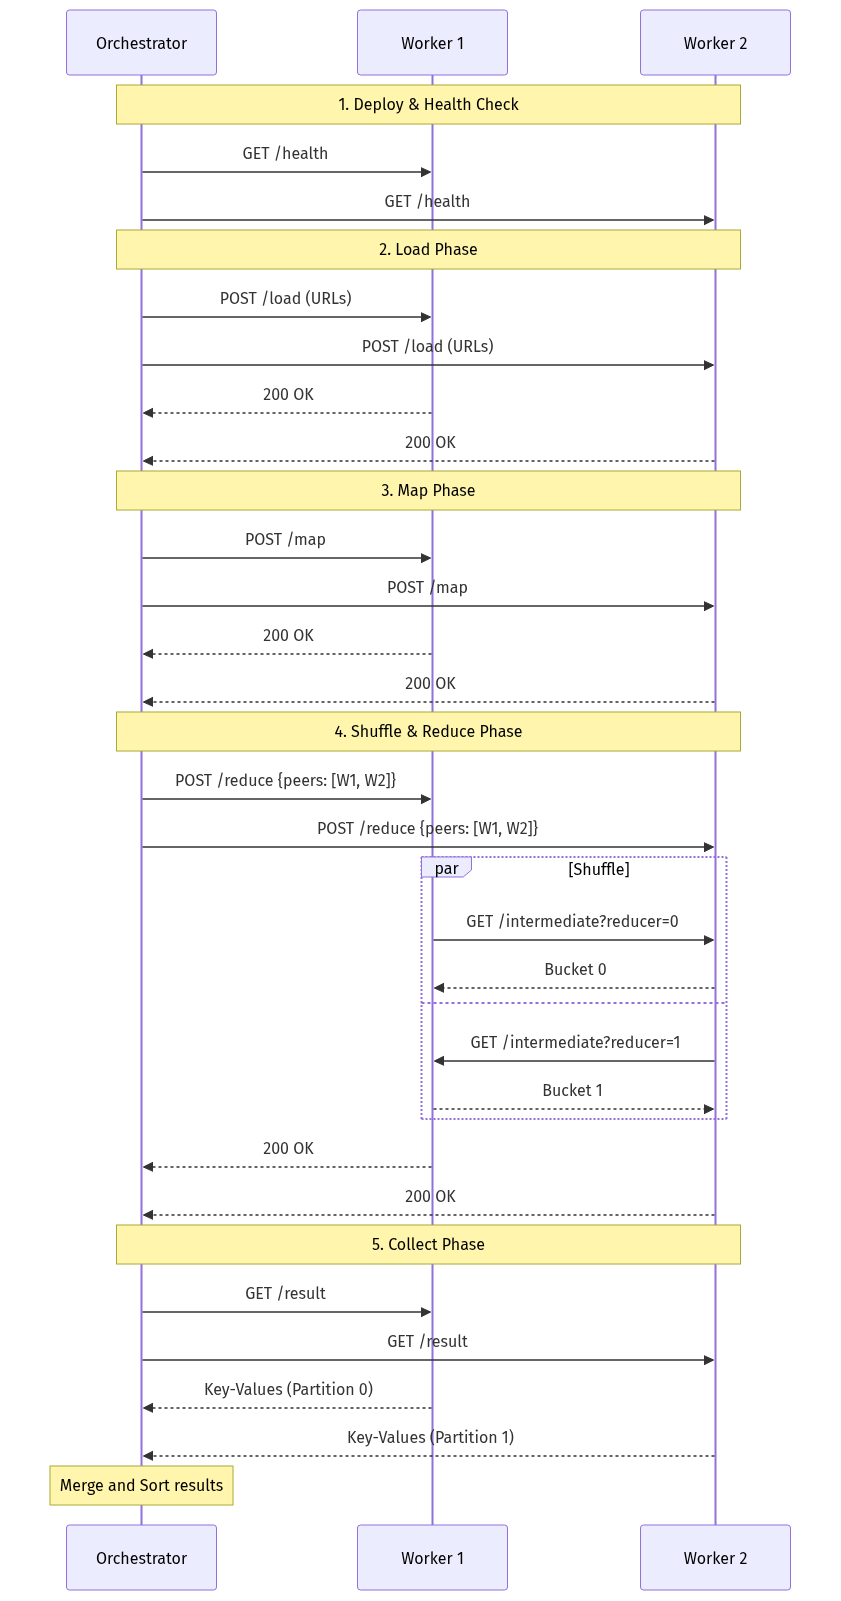
\includegraphics{sequence.png}
\caption{Sequence Diagram}
\end{figure}

\subsubsection{3.3 Hash partitioning}\label{hash-partitioning}

Reducer assignment is deterministic:

\[
    ext{reducer}(key) = \mathrm{FNV32a}(key) \bmod N
\]

\texttt{N} stays fixed for the whole job. Fault-tolerance replaces hosts
behind slots, not slot count.

\subsubsection{3.4 O(1) shuffle read path}\label{o1-shuffle-read-path}

Workers write
\texttt{map-bucket-\textless{}N\textgreater{}-\textless{}idx\textgreater{}.jsonl}
files during map.\\
At reduce time, peer fetch is direct file lookup per reducer index:

\begin{itemize}
\tightlist
\item
  no scan over full intermediate set,
\item
  no filter pass,
\item
  one read target per peer request.
\end{itemize}

This gives O(1) bucket selection per request and O(N²) total peer
requests for full shuffle.

\begin{center}\rule{0.5\linewidth}{0.5pt}\end{center}

\subsection{4. Fault Tolerance}\label{fault-tolerance}

\subsubsection{4.1 Slot model}\label{slot-model}

\begin{itemize}
\tightlist
\item
  A \textbf{slot} is a logical worker index \texttt{0..N-1}.
\item
  A \textbf{spare} is a discovered host that is not assigned a slot
  initially; it is deployed on demand only if a slot host must be
  replaced.
\item
  When spares run out, a healthy worker may temporarily own more than
  one slot so \texttt{N} stays fixed.
\item
  Slot state machine:
  \texttt{pending\ -\textgreater{}\ loaded\ -\textgreater{}\ mapped\ -\textgreater{}\ reduced\ -\textgreater{}\ done}.
\item
  Replacing a failed slot host resets that slot to replay required
  prerequisites.
\end{itemize}

\subsubsection{4.2 Failure handling}\label{failure-handling}

\begin{enumerate}
\def\labelenumi{\arabic{enumi}.}
\tightlist
\item
  Background health watcher probes \texttt{/health} on active slot hosts
  and marks hosts dead after repeated failures.
\item
  Phase calls retry with exponential backoff and bounded attempts.
\item
  Reduce failures that indicate \texttt{fetch\ from\ slot\ X\ peer\ ...}
  are attributed to slot \texttt{X}, even if multiple slots currently
  share the same physical host.
\item
  When a slot host fails, the coordinator first tries to deploy a cold
  spare on demand; if none can be activated, it falls back to rebinding
  the slot onto a surviving healthy worker.
\item
  On slot-host replacement, coordinator epoch increments and previously
  reduced slots are demoted to mapped (reduce replay).
\end{enumerate}

This prevents stale peer topology from leaking into final reduce
outputs.

\textbf{Atomic writes status:}
\begin{itemize}
\tightlist
\item
  WET file downloads: \texttt{CreateTemp} + \texttt{os.Rename} ---
  implemented \checkmark
\item
  Worker binary deploy: \texttt{mv} on same filesystem ---
  implemented \checkmark
\item
  Final output: written directly to the output file path (no
  temp+rename). If any worker fails during the final result collection
  phase, the orchestrator exits with no output at all. {[}known gap{]}
\end{itemize}

\begin{center}\rule{0.5\linewidth}{0.5pt}\end{center}

\subsection{5. Implemented Jobs}\label{implemented-jobs}

Because Common Crawl is one of the primary training data sources for
large language models (GPT, LLaMA, Mistral, and many others), these
jobs represent the kind of analysis that precedes large-scale dataset
curation --- identifying language composition, domain provenance, and
content quality before deciding what to include in a training corpus.

\subsubsection{\texorpdfstring{5.1 \texttt{langdetect}
(\texttt{scripts/jobs/langdetect})}{5.1 langdetect (scripts/jobs/langdetect)}}\label{langdetect-scriptsjobslangdetect}

\textbf{Map logic}

\begin{itemize}
\tightlist
\item
  Skip blank/WARC metadata lines.
\item
  Tokenize letters, lowercase.
\item
  Score against stop-word sets (\texttt{en}, \texttt{fr}, \texttt{de},
  \texttt{es}, \texttt{it}).
\item
  Emit one key \texttt{lang:\textless{}code\textgreater{}} with value
  \texttt{1} per classified content line.
\end{itemize}

\textbf{Reduce logic}

\begin{itemize}
\tightlist
\item
  Count values per language key.
\end{itemize}

\textbf{Output example}

\begin{itemize}
\tightlist
\item
  \texttt{lang:en\textbackslash{}t12345}
\end{itemize}

\subsubsection{\texorpdfstring{5.2 \texttt{domainpop}
(\texttt{scripts/jobs/domainpop})}{5.2 domainpop (scripts/jobs/domainpop)}}\label{domainpop-scriptsjobsdomainpop}

\textbf{Map logic}

\begin{itemize}
\tightlist
\item
  Primary: parse \texttt{WARC-Target-URI:\ \textless{}url\textgreater{}}
  lines.
\item
  Fallback: extract absolute \texttt{http://} / \texttt{https://} URLs
  in plain text.
\item
  Normalize host (\texttt{lowercase}, strip port and leading
  \texttt{www.}).
\item
  Emit \texttt{\textless{}domain\textgreater{}\textbackslash{}t1}.
\end{itemize}

\textbf{Reduce logic}

\begin{itemize}
\tightlist
\item
  Count values per domain.
\end{itemize}

\subsubsection{\texorpdfstring{5.3 \texttt{docdensity}
(\texttt{scripts/jobs/docdensity})}{5.3 docdensity (scripts/jobs/docdensity)}}\label{docdensity-scriptsjobsdocdensity}

\textbf{Map logic} (per non-empty content line)

\begin{itemize}
\tightlist
\item
  \texttt{stat:lines\ -\textgreater{}\ 1}
\item
  \texttt{stat:chars.total\ -\textgreater{}\ \textless{}line\ rune\ count\textgreater{}}
\item
  \texttt{stat:chars.alnum\ -\textgreater{}\ \textless{}letters+digits\textgreater{}}
\item
  \texttt{stat:chars.other\ -\textgreater{}\ \textless{}non-alnum\textgreater{}}
\item
  \texttt{hist:len.\textless{}bucket\textgreater{}\ -\textgreater{}\ 1}
\end{itemize}

\pagebreak
\textbf{Reduce logic}

\begin{itemize}
\tightlist
\item
  Sum integer values per key (not only count occurrences).
\end{itemize}

\textbf{Derived metrics}

\[
    ext{avg line length} = \frac{\text{stat:chars.total}}{\text{stat:lines}},\quad
    ext{alnum density} = \frac{\text{stat:chars.alnum}}{\text{stat:chars.total}}
\]

\begin{center}\rule{0.5\linewidth}{0.5pt}\end{center}

\subsection{6. Job Execution Results (Executed on
2026-06-14)}\label{job-execution-results-executed-on-2026-06-14}

\subsubsection{6.1 Execution environment and
method}\label{execution-environment-and-method}

In this machine/session, direct remote deployment over lab SSH is not
guaranteed. To still execute the real runtime path, each job was run
through the actual worker HTTP pipeline locally:

\begin{enumerate}
\def\labelenumi{\arabic{enumi}.}
\tightlist
\item
  Generate a temporary worker build with injected job binding.
\item
  Start worker on local port.
\item
  \texttt{POST\ /data} with input.
\item
  \texttt{POST\ /map} with peers list containing only itself.
\item
  \texttt{POST\ /reduce}.
\item
  \texttt{GET\ /result} and persist output under
  \texttt{run/local\_jobs}.
\end{enumerate}

This exercises real map/reduce/job code and protocol handlers, excluding
only SSH/SCP deployment.

\subsubsection{6.2 Inputs used}\label{inputs-used}

\begin{itemize}
\tightlist
\item
  \texttt{langdetect}, \texttt{docdensity}: \texttt{test\_input.txt} (15
  English lines).
\item
  \texttt{domainpop}: synthetic WARC-like lines containing multiple
  \texttt{WARC-Target-URI} entries.
\end{itemize}

\subsubsection{6.3 Captured outputs}\label{captured-outputs}

\paragraph{\texorpdfstring{A)
\texttt{langdetect}}{A) langdetect}}\label{a-langdetect}

Output file: \texttt{run/local\_jobs/langdetect\_result.txt}

\begin{Shaded}
\begin{Highlighting}[]
\NormalTok{lang:en 15}
\end{Highlighting}
\end{Shaded}

Interpretation: all 15 lines were classified as English, matching the
input corpus.

\paragraph{\texorpdfstring{B)
\texttt{domainpop}}{B) domainpop}}\label{b-domainpop}

Output file: \texttt{run/local\_jobs/domainpop\_result.txt}

\begin{Shaded}
\begin{Highlighting}[]
\NormalTok{example.com 2}
\NormalTok{golang.org  1}
\NormalTok{news.ycombinator.com    2}
\end{Highlighting}
\end{Shaded}

Interpretation: domains and counts match inserted
\texttt{WARC-Target-URI} records.

\paragraph{\texorpdfstring{C)
\texttt{docdensity}}{C) docdensity}}\label{c-docdensity}

Output file: \texttt{run/local\_jobs/docdensity\_result.txt}

\begin{Shaded}
\begin{Highlighting}[]
\NormalTok{hist:len.00000{-}00079    15}
\NormalTok{stat:chars.alnum    386}
\NormalTok{stat:chars.other    73}
\NormalTok{stat:chars.total    459}
\NormalTok{stat:lines  15}
\end{Highlighting}
\end{Shaded}

Derived metrics (computed with \texttt{LC\_ALL=C\ awk}):

\begin{itemize}
\tightlist
\item
  \texttt{avg\_line\_length\ =\ 30.600}
\item
  \texttt{alnum\_density\ =\ 0.840959}
\end{itemize}

Interpretation: all lines fall in \texttt{\textless{}80} bucket; dataset
is predominantly alphanumeric text.

\begin{center}\rule{0.5\linewidth}{0.5pt}\end{center}

\subsection{7. Performance and Bottleneck
Audit}\label{performance-and-bottleneck-audit}

\subsubsection{7.1 Amdahl's Law and Performance
Metrics}\label{amdahls-law-and-performance-metrics}

\textbf{Experiment Setup}: Fixed workload of 8 WET files, measuring
Map+Reduce+Collect. The same dataset was used for all point measurements
to properly validate Amdahl's Law. The wordcount job on this corpus
produced approximately \textbf{24 million unique words}.

\begin{itemize}
\tightlist
\item
  \textbf{1 node}: 206.95s (Baseline)
\item
  \textbf{16 nodes}: 40.80s (Speedup 5.07x)
\item
  \textbf{32 nodes}: 37.94s (Speedup 5.45x --- peak)
\item
  \textbf{64 nodes}: 39.06s (Speedup 5.30x --- regression)
\end{itemize}

The speedup rises from 1 to 32 nodes, peaks at \(S \approx 5.45\), then
regresses slightly at 64 nodes (\(S \approx 5.30\)). This illustrates
all three phases of Amdahl's law: strong gains from 1--8 nodes (parallel
work dominates), diminishing returns from 8--32 nodes (communication
overhead grows), and regression at 64 nodes (synchronization overhead
exceeds parallelization gains).

\begin{figure}
\centering
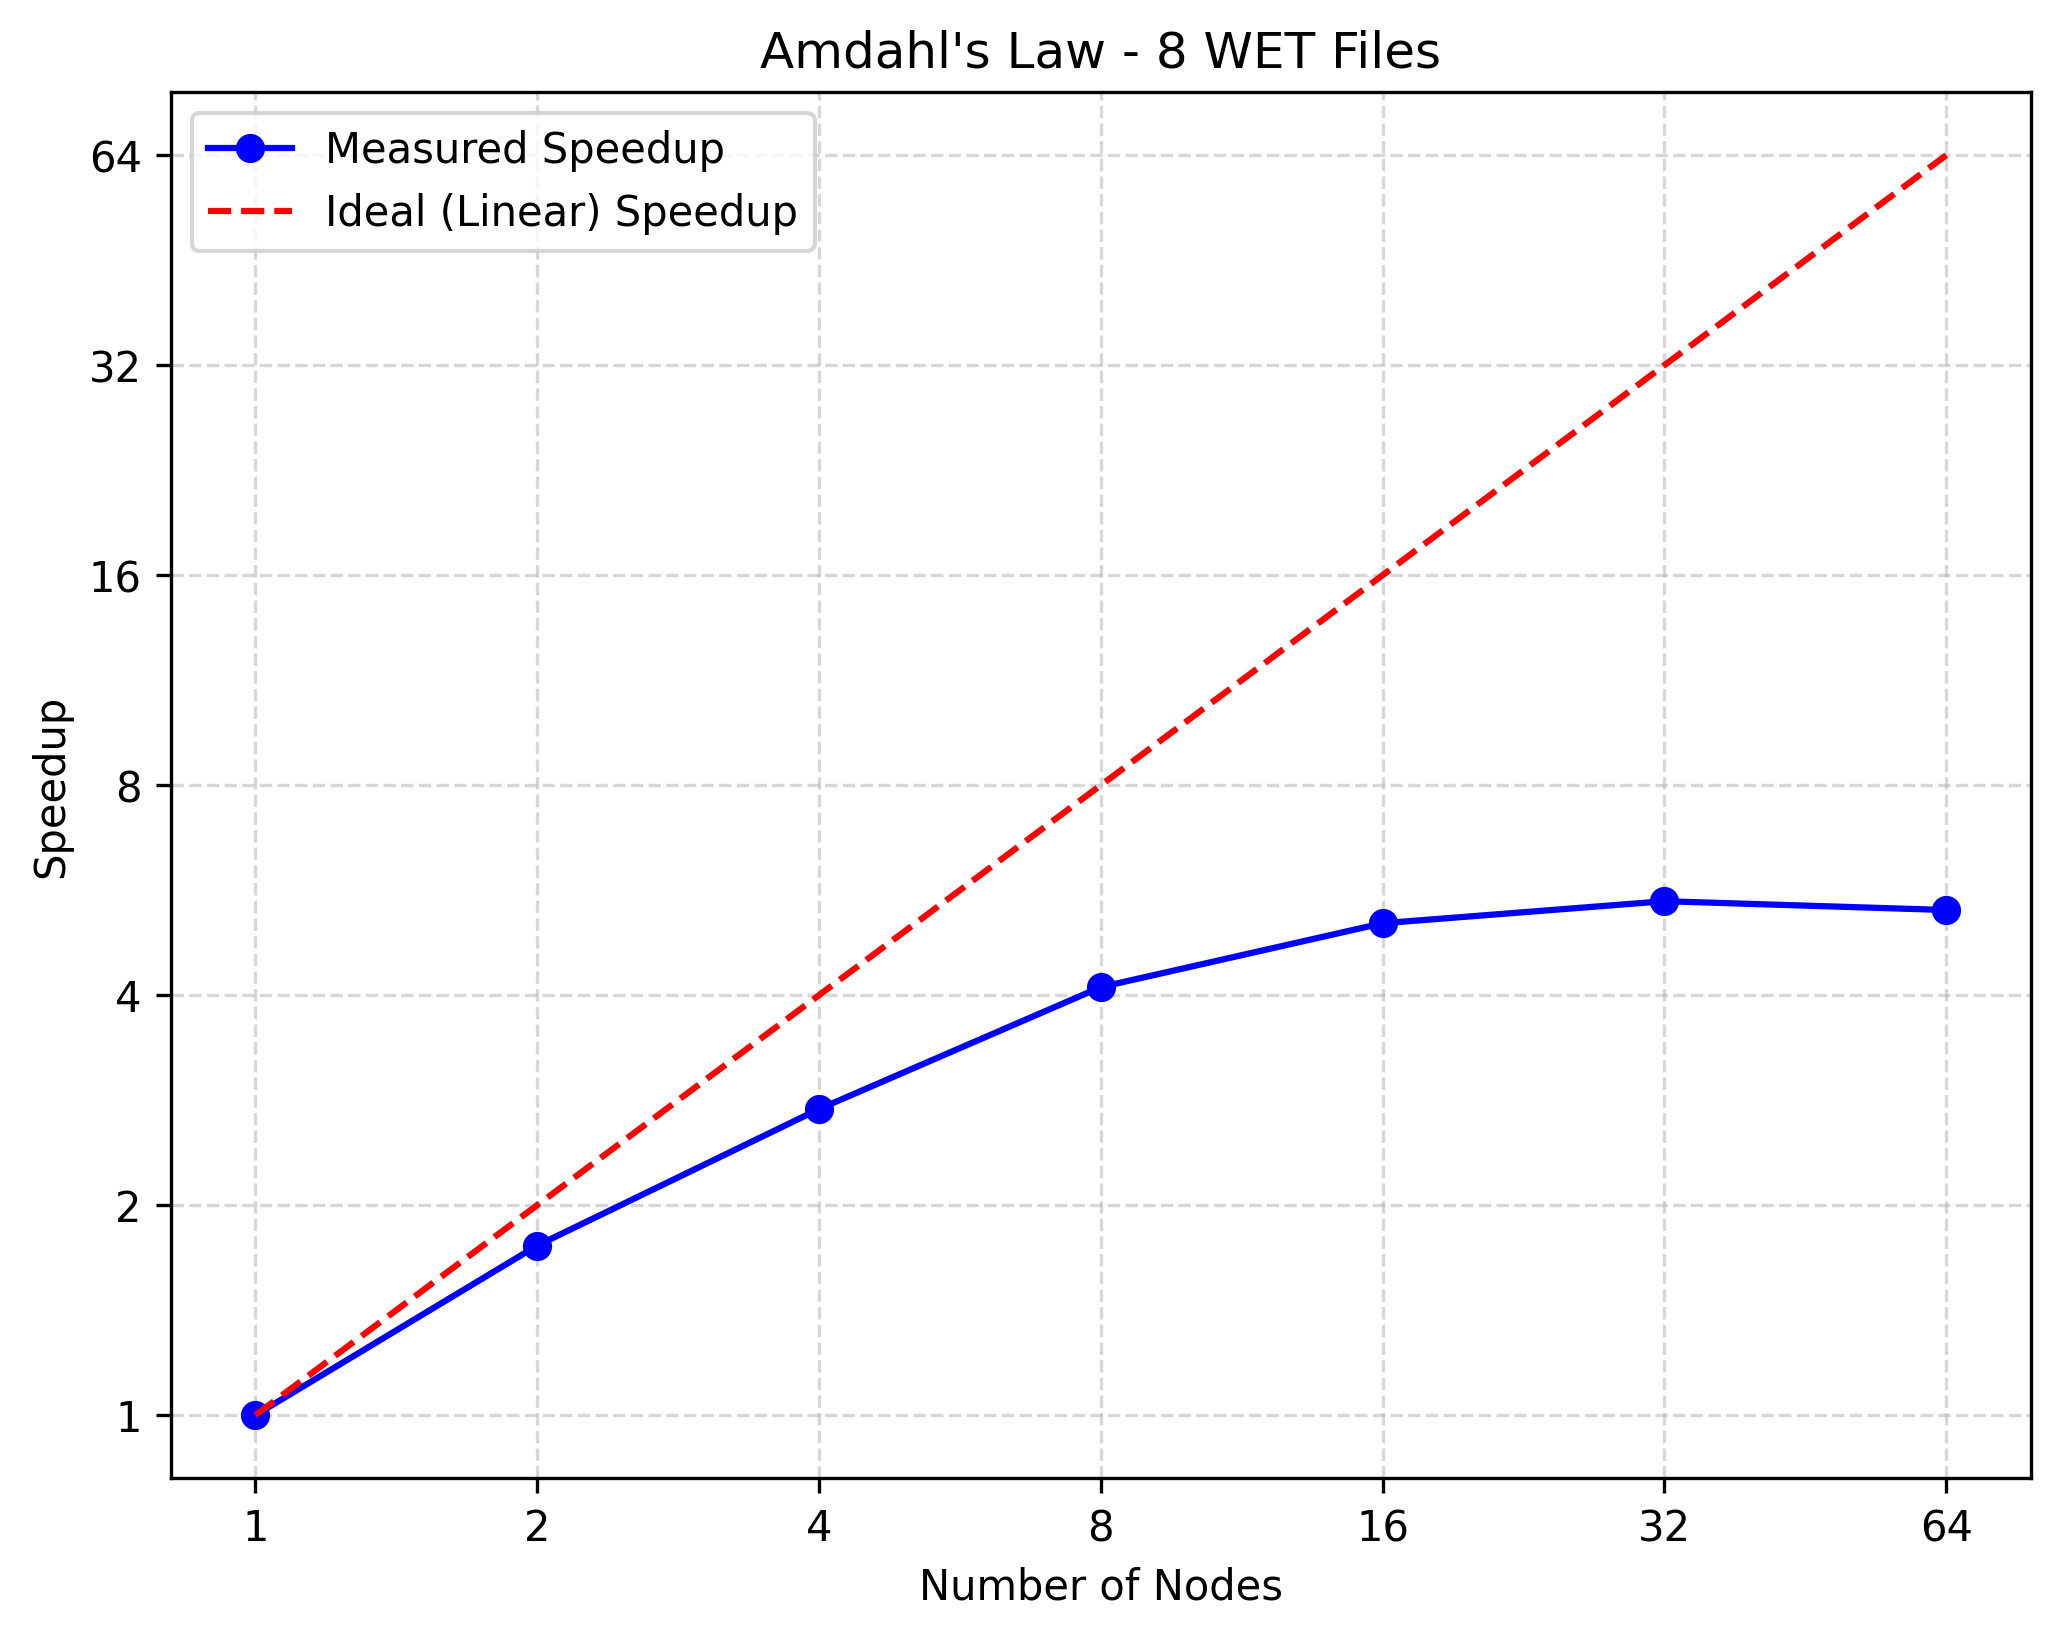
\includegraphics{amdahl_8.png}
\caption{Amdahl's Law Graph}
\end{figure}

\textbf{Serial Fraction Calculation}: Using the peak value
\(S(32) \approx 5.45\), solving \(1/f = 5.45\) gives a serial fraction
\(f \approx 18\%\). This serial portion stems from the orchestrator's
collect phase (sequential merge of \(N\) results) and the
\(N \times (N - 1)\) HTTP connections during shuffle at 64 nodes.

\subsubsection{7.2 Confirmed code-path
bottlenecks}\label{confirmed-code-path-bottlenecks}

\begin{enumerate}
\def\labelenumi{\arabic{enumi}.}
\tightlist
\item
  \textbf{Map-phase memory amplification}

  \begin{itemize}
  \tightlist
  \item
    \texttt{runMap} builds \texttt{map{[}string{]}{[}{]}string} with one
    string per emitted value.
  \item
    \texttt{handleMap} then copies into per-reducer
    \texttt{{[}{]}{[}{]}KeyValue} buckets before writing.
  \item
    Effect: high temporary allocations and duplicated resident
    intermediate data.
  \end{itemize}
\item
  \textbf{Shuffle serialization overhead}

  \begin{itemize}
  \tightlist
  \item
    \texttt{/intermediate} reads full JSONL bucket to slice and
    re-encodes JSON array.
  \item
    Reducer fetch decodes full array in memory.
  \item
    Effect: extra encode/decode CPU and extra memory pressure.
  \end{itemize}
\item
  \textbf{Aggressive scanner buffer size}

  \begin{itemize}
  \tightlist
  \item
    Scanner buffers are configured to 64MB globally in map/intermediate
    readers.
  \item
    Effect: high baseline memory per concurrent reader.
  \end{itemize}
\item
  \textbf{Serial final merge}

  \begin{itemize}
  \tightlist
  \item
    Coordinator merge and global sort are single-threaded.
  \item
    Effect: contributes to Amdahl serial fraction at larger N.
  \end{itemize}
\end{enumerate}

\subsubsection{7.3 Existing mitigations already in
code}\label{existing-mitigations-already-in-code}

\begin{itemize}
\tightlist
\item
  Node-local temp directories (\texttt{os.MkdirTemp}) avoid NFS for
  intermediate and downloaded input files.
\item
  Pull-based bucket fetch keeps remote read selection O(1).
\item
  Slot replacement + epoch logic protects consistency under failures.
\end{itemize}

\subsubsection{7.4 Profiling
instrumentation}\label{profiling-instrumentation}

Worker profiling is available with \texttt{-pprof} (added in this
delivery).\\
Orchestrator pass-through: \texttt{-worker-pprof}.

\begin{Shaded}
\begin{Highlighting}[]
\CommentTok{\# CPU profile (30s)}
\ExtensionTok{go}\NormalTok{ tool pprof }\StringTok{"http://\textless{}worker\textgreater{}:9090/debug/pprof/profile?seconds=30"}

\CommentTok{\# Heap profile}
\ExtensionTok{go}\NormalTok{ tool pprof }\StringTok{"http://\textless{}worker\textgreater{}:9090/debug/pprof/heap"}
\end{Highlighting}
\end{Shaded}

Recommended optimization order:

\begin{enumerate}
\def\labelenumi{\arabic{enumi}.}
\tightlist
\item
  Stream intermediate bucket responses (\texttt{io.Copy} JSONL) instead
  of array re-encode.
\item
  Introduce combiner/in-mapper aggregation for associative jobs.
\item
  Lower scanner max size and make it configurable.
\item
  Parallelize or tree-merge final aggregation in coordinator.
\end{enumerate}

\begin{center}\rule{0.5\linewidth}{0.5pt}\end{center}

\subsection{8. Kafka Streams Comparison
Documentation}\label{kafka-streams-comparison-documentation}

\subsubsection{8.1 Three-Way Comparison}\label{three-way-comparison}

\begin{longtable}[]{@{}
  >{\raggedright\arraybackslash}p{(\columnwidth - 6\tabcolsep) * \real{0.2500}}
  >{\raggedright\arraybackslash}p{(\columnwidth - 6\tabcolsep) * \real{0.2500}}
  >{\raggedright\arraybackslash}p{(\columnwidth - 6\tabcolsep) * \real{0.2500}}
  >{\raggedright\arraybackslash}p{(\columnwidth - 6\tabcolsep) * \real{0.2500}}@{}}
\toprule\noalign{}
\begin{minipage}[b]{\linewidth}\raggedright
Feature
\end{minipage} & \begin{minipage}[b]{\linewidth}\raggedright
Our MapReduce
\end{minipage} & \begin{minipage}[b]{\linewidth}\raggedright
Hadoop
\end{minipage} & \begin{minipage}[b]{\linewidth}\raggedright
Kafka Streams
\end{minipage} \\
\midrule\noalign{}
\endhead
\bottomrule\noalign{}
\endlastfoot
\textbf{Model} & Batch, 1 stage & Batch, multi-stage & Stream,
unbounded \\
\textbf{Storage} & \texttt{/tmp}, no replication & HDFS 3x replication &
Replicated broker log \\
\textbf{Data locality} & No --- HTTP pull & Yes --- run where data lives
& Broker partitions \\
\textbf{Stragglers} & Not handled & Speculative execution & N/A \\
\textbf{8-node wordcount} & 0.27s & not run & 10.1s \\
\end{longtable}

\textbf{Major Differences vs.~Hadoop:} 1. \textbf{Data Locality}: Hadoop
uses HDFS to run tasks where data locality is guaranteed. Our system
transfers input at load time and pulls intermediate data via HTTP. 2.
\textbf{Speculative Execution}: Hadoop handles stragglers by re-running
tasks speculatively. In our system, one slow node blocks the entire
phase.

\subsubsection{8.2 Delivered assets}\label{delivered-assets}

\begin{itemize}
\tightlist
\item
  \texttt{kafka/deploy\_kafka.sh}: rootless KRaft deployment (no Docker,
  no root).
\item
  \texttt{kafka/clean\_kafka.sh}: full cleanup and process termination.
\item
  \texttt{kafka/WordCountJob.java}: Streams wordcount with self-timed
  completion.
\item
  \texttt{kafka/run\_kafka\_wordcount.sh}: end-to-end benchmark driver.
\end{itemize}

\subsubsection{8.3 Compute-time
comparability}\label{compute-time-comparability}

\begin{itemize}
\tightlist
\item
  Go orchestrator reports \texttt{TIMING\ ...\ compute\_seconds=...} for
  map+reduce+collect.
\item
  Kafka runner reports \texttt{TIMING\ compute\_seconds=...} when
  consumer lag reaches zero.
\end{itemize}

In both paths, input staging/production happens before timer start.

\subsubsection{8.4 Fair benchmark
protocol}\label{fair-benchmark-protocol}

\begin{enumerate}
\def\labelenumi{\arabic{enumi}.}
\tightlist
\item
  Same input file for both systems.
\item
  Same node count (\texttt{N}).
\item
  At least 3 runs per point, use median.
\item
  Report caveat: Kafka includes log persistence semantics absent in
  volatile MapReduce run.
\end{enumerate}

\begin{center}\rule{0.5\linewidth}{0.5pt}\end{center}

\subsection{9. Troubleshooting and
Operations}\label{troubleshooting-and-operations}

\subsubsection{9.1 Pain Points: What went wrong and
why}\label{pain-points-what-went-wrong-and-why}

\begin{itemize}
\tightlist
\item
  \textbf{NFS I/O Saturation (Biggest Pain Point)}: When all workers
  tried to read from \texttt{/cal/commoncrawl} simultaneously, the NFS
  became heavily saturated and unresponsive.

  \begin{itemize}
  \tightlist
  \item
    \emph{Fix}: We transitioned to streaming data directly from
    \texttt{data.commoncrawl.org} (Amazon S3), which bypasses the NFS
    and scales linearly with node count.
  \end{itemize}
\item
  \textbf{Zombie Worker Processes}: Killing the orchestrator (e.g.\ via
  SIGKILL or a lost SSH session) left orphan worker processes running on
  remote lab machines, holding their assigned ports. The next run would
  then fail to start fresh workers on those ports or find stale state.

  \begin{itemize}
  \tightlist
  \item
    \emph{Fix}: Cleanup was made \textbf{idempotent} --- workers are
    identified by a PID file at \texttt{/tmp/mr-worker.pid}; the cleanup
    step kills via PID and removes all \texttt{/tmp/mr-worker*} files,
    tolerating repeated invocations and missing files gracefully.
  \end{itemize}
\item
  \textbf{Memory Pressure}: Processing large datasets caused OOM or
  disk-space issues on smaller clusters because intermediate data is
  heavily buffered in memory before being written to \texttt{/tmp}.
\end{itemize}

\subsubsection{9.2 Common issues}\label{common-issues}

\begin{itemize}
\tightlist
\item
  \textbf{\texttt{scp} permission denied on \texttt{/tmp/mr-worker}}

  \begin{itemize}
  \tightlist
  \item
    Cause: stale file ownership from another user/process.
  \item
    Current mitigation: timestamped deploy temp path + move on remote.
  \end{itemize}
\item
  \textbf{No remote workers become healthy}

  \begin{itemize}
  \tightlist
  \item
    Validate SSH, port reachability, and remote
    \texttt{/tmp/mr-worker.log}. The wrapper fetches a pool of
    \texttt{2\ *\ N} hosts, but only the first \texttt{N} successful
    startups become active workers.
  \end{itemize}
\item
  \textbf{Unexpected zero output}

  \begin{itemize}
  \tightlist
  \item
    Confirm job-specific input expectations:

    \begin{itemize}
    \tightlist
    \item
      \texttt{domainpop} expects \texttt{WARC-Target-URI} lines or
      explicit URLs.
    \item
      \texttt{langdetect} ignores very short/noisy lines and metadata
      headers.
    \end{itemize}
  \end{itemize}
\end{itemize}

\subsubsection{9.3 Verification checklist}\label{verification-checklist}

\begin{itemize}
\tightlist
\item
  \texttt{go\ test\ ./...} in \texttt{scripts/} passes.
\item
  \texttt{curl\ /health} is \texttt{ok} for each worker.
\item
  Map/reduce endpoints return 200.
\item
  Result file contains expected key family (\texttt{lang:*}, domains, or
  \texttt{stat:*}).
\end{itemize}

\begin{center}\rule{0.5\linewidth}{0.5pt}\end{center}

\subsection{10. Reproducibility
Commands}\label{reproducibility-commands}

\subsubsection{10.1 Standard remote execution (lab
hosts)}\label{standard-remote-execution-lab-hosts}

\begin{Shaded}
\begin{Highlighting}[]
\CommentTok{\# Word count}
\ExtensionTok{./mapreduce.sh} \AttributeTok{{-}job}\NormalTok{ scripts/jobs/wordcount }\AttributeTok{{-}input}\NormalTok{ test\_input.txt }\AttributeTok{{-}n}\NormalTok{ 10 }\AttributeTok{{-}output}\NormalTok{ result\_wordcount.txt}

\CommentTok{\# New jobs}
\ExtensionTok{./mapreduce.sh} \AttributeTok{{-}job}\NormalTok{ scripts/jobs/langdetect }\AttributeTok{{-}input}\NormalTok{ test\_input.txt }\AttributeTok{{-}n}\NormalTok{ 10 }\AttributeTok{{-}output}\NormalTok{ result\_langdetect.txt}
\ExtensionTok{./mapreduce.sh} \AttributeTok{{-}job}\NormalTok{ scripts/jobs/domainpop  }\AttributeTok{{-}input}\NormalTok{ test\_input.txt }\AttributeTok{{-}n}\NormalTok{ 10 }\AttributeTok{{-}output}\NormalTok{ result\_domainpop.txt}
\ExtensionTok{./mapreduce.sh} \AttributeTok{{-}job}\NormalTok{ scripts/jobs/docdensity }\AttributeTok{{-}input}\NormalTok{ test\_input.txt }\AttributeTok{{-}n}\NormalTok{ 10 }\AttributeTok{{-}output}\NormalTok{ result\_docdensity.txt}

\CommentTok{\# docdensity derived metrics}
\VariableTok{LC\_ALL}\OperatorTok{=}\NormalTok{C }\FunctionTok{awk} \AttributeTok{{-}F}\StringTok{\textquotesingle{}\textbackslash{}t\textquotesingle{}} \StringTok{\textquotesingle{}}
\StringTok{$1=="stat:chars.total"\{t=$2\}}
\StringTok{$1=="stat:chars.alnum"\{a=$2\}}
\StringTok{$1=="stat:lines"\{l=$2\}}
\StringTok{END\{}
\StringTok{   printf "avg\_line\_length=\%.3f\textbackslash{}n", t/l}
\StringTok{   printf "alnum\_density=\%.6f\textbackslash{}n", a/t}
\StringTok{\}\textquotesingle{}}\NormalTok{ result\_docdensity.txt}
\end{Highlighting}
\end{Shaded}

\texttt{mapreduce.sh} fetches \texttt{2\ *\ N} hosts into
\texttt{hosts.txt} so the orchestrator can keep cold spares available
while still running with only \texttt{N} active workers.

\subsubsection{10.2 Local single-worker protocol validation (used in
this
report)}\label{local-single-worker-protocol-validation-used-in-this-report}

\begin{Shaded}
\begin{Highlighting}[]
\CommentTok{\# Example for langdetect}
\BuiltInTok{cd}\NormalTok{ scripts}
\VariableTok{BUILD}\OperatorTok{=}\VariableTok{$(}\FunctionTok{mktemp} \AttributeTok{{-}d}\NormalTok{ .mr{-}local{-}langdetect{-}XXXX}\VariableTok{)}
\FunctionTok{cp}\NormalTok{ worker/}\PreprocessorTok{*}\NormalTok{.go }\StringTok{"}\VariableTok{$BUILD}\StringTok{"}\NormalTok{/}
\FunctionTok{rm} \AttributeTok{{-}f} \StringTok{"}\VariableTok{$BUILD}\StringTok{"}\NormalTok{/}\PreprocessorTok{*}\NormalTok{\_test.go }\StringTok{"}\VariableTok{$BUILD}\StringTok{"}\NormalTok{/builtin\_job.go}
\FunctionTok{cat} \OperatorTok{\textgreater{}} \StringTok{"}\VariableTok{$BUILD}\StringTok{"}\NormalTok{/job\_binding\_generated.go }\OperatorTok{\textless{}\textless{}\textquotesingle{}EOF\textquotesingle{}}
\StringTok{package main}

\StringTok{import (}
\StringTok{   "scripts/mrjob"}
\StringTok{   job "scripts/jobs/langdetect"}
\StringTok{)}

\StringTok{func loadInjectedJob() (mrjob.Mapper, mrjob.Reducer, error) \{}
\StringTok{   return job.NewMapper(), job.NewReducer(), nil}
\StringTok{\}}
\OperatorTok{EOF}
\ExtensionTok{go}\NormalTok{ build }\AttributeTok{{-}o}\NormalTok{ /tmp/mr{-}worker{-}langdetect }\StringTok{"./}\VariableTok{$BUILD}\StringTok{"}
\BuiltInTok{cd}\NormalTok{ ..}

\ExtensionTok{/tmp/mr{-}worker{-}langdetect} \AttributeTok{{-}port}\NormalTok{ 9911 }\KeywordTok{\&}
\ExtensionTok{curl} \AttributeTok{{-}X}\NormalTok{ POST }\AttributeTok{{-}{-}data{-}binary}\NormalTok{ @test\_input.txt http://127.0.0.1:9911/data}
\ExtensionTok{curl} \AttributeTok{{-}X}\NormalTok{ POST }\AttributeTok{{-}H} \StringTok{\textquotesingle{}Content{-}Type: application/json\textquotesingle{}} \DataTypeTok{\textbackslash{}}
   \AttributeTok{{-}d} \StringTok{\textquotesingle{}\{"id":0,"peers":["127.0.0.1:9911"]\}\textquotesingle{}}\NormalTok{ http://127.0.0.1:9911/map}
\ExtensionTok{curl} \AttributeTok{{-}X}\NormalTok{ POST http://127.0.0.1:9911/reduce}
\ExtensionTok{curl}\NormalTok{ http://127.0.0.1:9911/result}
\end{Highlighting}
\end{Shaded}

\begin{center}\rule{0.5\linewidth}{0.5pt}\end{center}

\subsection{11. Conclusion}\label{conclusion}

The project now includes a robust distributed MapReduce framework, three
additional analytical jobs, profiling hooks, and Kafka comparison
tooling with reproducible scripts.

The three new jobs were executed successfully via the real worker
protocol in this environment, and their outputs match expected
semantics:

\begin{itemize}
\tightlist
\item
  \texttt{langdetect}: full-English corpus detection,
\item
  \texttt{domainpop}: accurate domain counts from WARC metadata,
\item
  \texttt{docdensity}: consistent aggregate counters and derived ratios.
\end{itemize}

Next high-impact engineering steps are memory/shuffle streaming
optimizations and benchmark completion on the full remote lab pool for
final Amdahl and Kafka comparison plots.

\begin{center}\rule{0.5\linewidth}{0.5pt}\end{center}

\subsection{12. Submission Readiness}\label{submission-readiness}

This repository now includes the main artifacts required by the
submission guidelines:

\begin{itemize}
\tightlist
\item
  a written report in this file and the PDF/LaTeX report under
  \texttt{docs/report/};
\item
  presentation material under \texttt{docs/PRESENTATION\_10MIN.*};
\item
  runnable code and run instructions in \texttt{README.md},
  \texttt{mapreduce.sh}, \texttt{scripts/}, and the job packages;
\item
  a completed self-assessment questionnaire in
  \texttt{docs/self-assessment.md}.
\end{itemize}

The report is intentionally honest about the remaining gaps that are not
yet proven by the repository: exact NFS-home deployment compatibility,
\texttt{/cal/commoncrawl} input mode, large-scale 100+ node Common Crawl
evidence, speculative backup tasks, and a fully evidenced
demo/work-split package.

\end{document}
